%%%%%%%%%%%%%%%%%%%%%%%%%%%%%%%%%%%%%%%%%%%%%%%%%%%%%%%%%%%%%%%%%%%
\section{Constraint-based Score as Target Function in Bayesian Optimization Approach}

+ Explain the internal step in BayOpt.
Can make use some figures Fig.~\ref{fig:bayopt5}, Fig.\ref{fig:bayopt10}.

\begin{figure}
\centering
\includegraphics[scale=0.25]{{ucb_kappa5_constraint1.0_DIGITS_step5}.png}
\caption{BayOpt after 5 steps.}\label{fig:bayopt5}
\end{figure}


\begin{figure}
\centering
\includegraphics[scale=0.25]{{ucb_kappa5_constraint1.0_DIGITS_step10}.png}
\caption{BayOpt after 10 steps.}\label{fig:bayopt10}
\end{figure}

+ Explain how the utility function are constructed and optimized, and answer why optimize the utility function (surrogate function), we can optimize at the same time the target function (the constraint-based score function).

+ Explain the exploitation-exploration trade-off in BayOpt (and estimate the number of times we need to try before reaching to the global maximum).

%+ Note about the nature of BayOpt that, it can work with any non-convex multi-modal objective function and it assures to find the global extremum.


%%%%%%%%%%%%%%%%%%%%%%%%%%%%%%%%%%%%%%%%%%%%%%%%%%%%%%%%%%%%%%%%%%%%%%%%%%%%%%%%%%%%%%%%%%%%%%%
\section{Experimental Setups}\label{sec:XP}


\subsection{Presentation of the Experimental Datasets}

In our experiments, datasets with very different properties are used. The six used datasets are summaries in Table~\ref{tbl:dataset}.
\emph{DIGITS} is a subset of the optical recognition of handwritten digits dataset~\cite{kaynak1995methods} of 8x8 grayscale images.
\emph{COIL20} \cite{nene1996} is a dataset of 32x32 grayscale pictures of 20 rotated objects.
\emph{FASHION\_1K} contains 1000 grayscale images of size 28x28, sampled from Fashion-MNIST\cite{xiao2017/online} clothing dataset.
The grayscale images from these datasets are normalized and used directly in the DR methods.

\emph{FASHION\_MOBILENET} contains features extracted from a subset of the Fashion Product images dataset~\cite{fashionproduct}.
In order to construct this dataset, MobileNet~\cite{} with pre-trained weights from ImageNet is used for feature extraction. This transfer learning technique uses the representation of the learned network (trained on a large-scale image classification task) to extract meaningful features for new samples.
The last fully connected layer of the network is replaced by a global average pooling layer~\cite{} to obtain the flatten output vector of 1280 dimensions.
To speed up the DR methods, PCA is then applied to consider only 75 features.

\emph{5NEWS} contains the text of 5 groups selected from the 20 Newsgroups dataset, which are converted to a matrix of token counts via the TF-IDF method.
The count vectors are then fed into Latent Dirichlet Allocation (LDA) model to extract 15 hidden topics, which are the 15 features used by DR methods.

The \emph{NEURON\_1K}~\cite{neuron1k} dataset contains 1301 Brain Cells from an E18 Mouse, processed and provided by 10X Genomics, a company who provides chromium single cell gene expression solution and makes available several genetic datasets\footnote{https://www.10xgenomics.com/resources/datasets/; The datasets are licensed under the Creative Commons Attribution license.}.
The processed data have 10 PCA features and contains 6 labels that have been found by a graph-based clustering method.

\begin{table*}%[width=\textwidth,cols=6,pos=h]
\caption{Description of six selected datasets with samples for the image datasets.}\label{tbl:dataset}
\begin{tabular}{m{3cm} m{4.8cm} m{8cm}}
\toprule
Dataset name & Samples & Description \\
\midrule

\emph{COIL20}
    & 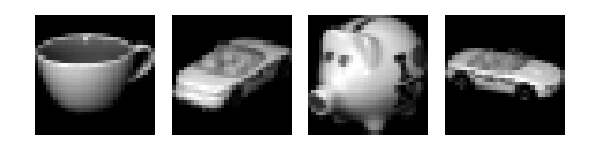
\includegraphics[width=\linewidth]{COIL20_samples}
    & 1440 grayscale images of size 32x32, belonging to 20 classes.
    The raw images of 1024 dimensions are used directly for the DR methods.\\

\emph{DIGITS}
    & 
\includegraphics[width=\linewidth]{DIGITS_samples}
    & 1797 grayscale images of size 8x8 of 10 digits.
    The raw images of 64 dimensions are used directly for the DR methods.\\

\emph{FASHION\_1K}
    & 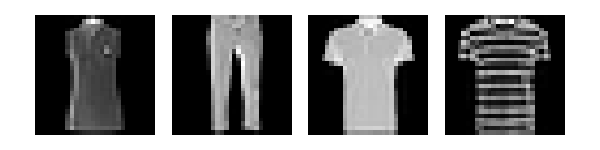
\includegraphics[width=\linewidth]{FASHION1000_samples}
    & 1000 grayscale images of size 28x28 of 10 classes, sampled from Fashion-MNIST dataset.
    The raw images of 768 dimensions are used directly for the DR methods.\\

\emph{FASHION\_MOBILENET}
    & 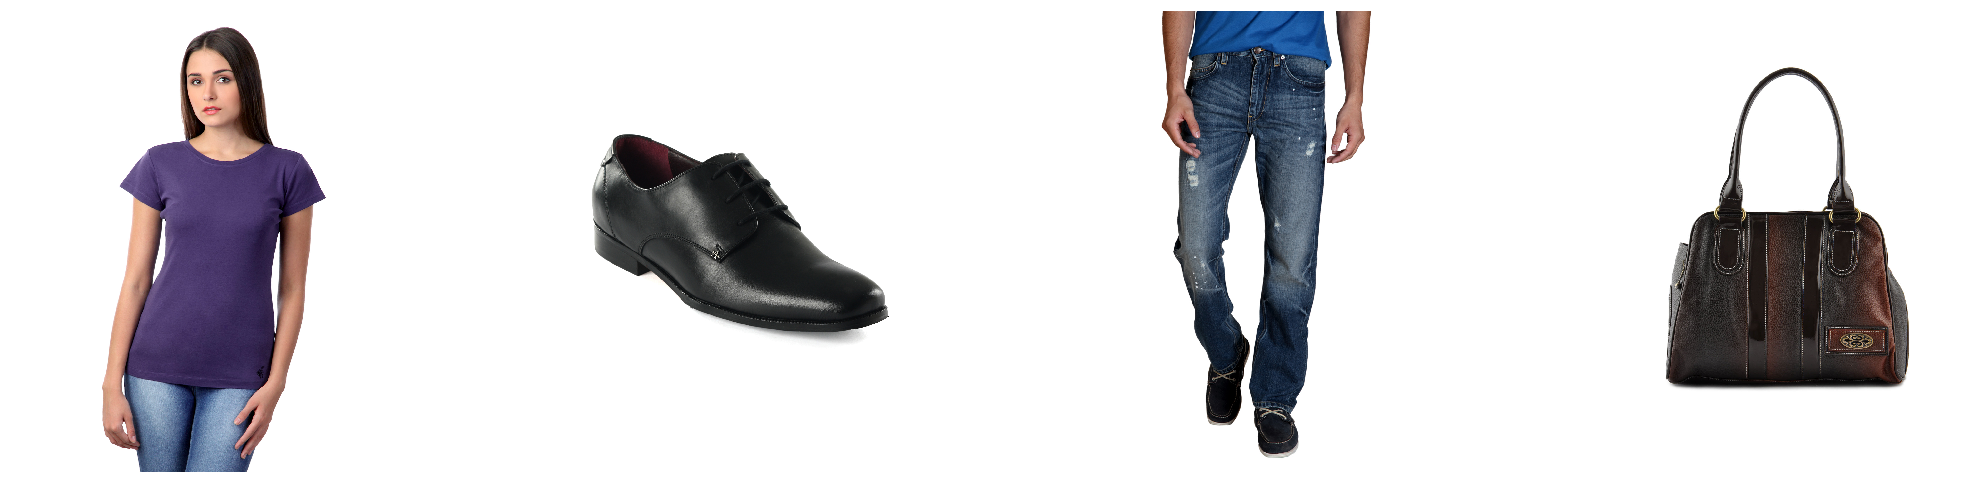
\includegraphics[width=\linewidth]{FASHION_PRODUCT_samples}
    & 1494 color images of various sizes belonging to 7 classes
    (\verb|'Bags', 'Bottomwear', 'Jewellery', 'Sandal', 'Shoes', 'Topwear', 'Watches'|),
    sampled from Fashion Product images dataset.\\

\emph{5NEWS}
    & 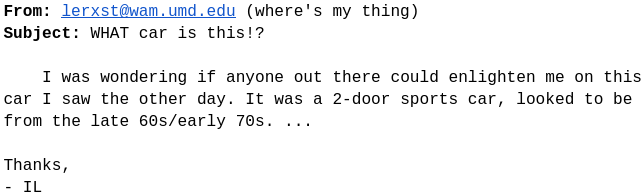
\includegraphics[width=\linewidth]{20NEWS5_samples}
    & 5 groups of 2957 emails selected from 20Newsgroups dataset,
    including \verb|'rec.autos', 'rec.sport.baseball','sci.crypt', 'sci.space', 'comp.sys.mac.hardware'|. \\

\emph{NEURON\_1K}
    &
    & 1301 brain cells from a combined cortex, hippocampus and subventricular zone of an E18 mouse. \\

\bottomrule
\end{tabular}
\end{table*}


\subsection{Constraint Generation}\label{subsec:constraint_generation}

The input for our proposed constraint preserving scores is ensemble of constraints in form of similar links and dissimilar links.


\subsection{Proof of Concept}


For the flexibility:
We design the score independently to the DR methods.
As shown in the above experiments, the constraint score can be used to evaluate the embedding quality of t-SNE or UMAP.
These well-known methods are widely used since they have ability to preserve the neighborhood information, i.e. to make the data points in the same class close together.
In this way, the local structure of the data is highlighted.
But as pointed out in the distill article ``How to use t-sne effectively'' by \citet{wattenberg2016use}, the distance between clusters might not mean anything.

The hyperparameters of t-SNE and UMAP make these methods difficult to use correctly but also make them flexible.
These methods can produce different visualizations and reveal different hidden structures in the data.
To evaluate the embedding quality of such flexible methods, we need a flexible score.
The state of the art $AUC_{log}RNX$ metric or the BIC-based score has no flexibility to capture different visualization results.

$AUC_{log}RNX$ metric evaluates how the neighborhood information is preserved.
The BIC-based score evaluates the trade-off between KL loss and the value of perplexity in t-SNE.
In contrast, the $f_{score}$ evaluates how the constraints are preserved.

$f_{score}$ takes a set of constraints as input to find the best visualization which respects the constraints.
Naturally, the constraints generated from the class labels reflect the class-relationship between the data points in the same class.



%%%%%%%%%%%%%%%%%%%%%%%%%%%%%%%%%%%%%%%%%%%%%%%%%%%%%%%%%%%%%%%%%%%%%%%%%%%%%%%%%%%%%%%%%%%%%%%
\section{Experimental Results}\label{sec:results}



%%%%%%%%%%%%%%%%%%%%%%%%%%%%%%%%%%%%%%%%%%%%%%%%%%%%%%%%%%%%%%%%%%%%%%%%%%%%%%%%%%%%%%%%%%%%%%%
\section{Discussion}\label{sec:discussion}

\par
Discuss the variance of the proposed score (w.r.t to different set of constraints, different number of constraitns).
Say, the constraint-based score is a stochastic function.
Say, how BayOpt can take into account the uncertainty (the variance of the score) to estimate the maximum of this stochastic function.


\par
The violated constraints in our methods correspond to the shortcomming of t-SNE in \cite{wattenberg2016use}.
t-SNE can not preserve the within-cluster distances and between-clusters distances.
[TODO: Add reproduced figures].
The $q_{ij}$-based score can help to understand the defective of the visualization.

\par
Add discussion for UMAP.

\par
Easily generate pairwise constraints from labels.
  Only need small amount of labeled points for each class to generate hundreds of constraints.
  The proposed method only need 200 constraints to work well.
  [TODO: Test with smaller number of constraints to see if it works. 200 constraints seem too much].

\par
Can replace the auto-generated constraints by the manual constraints of the real user.

\par
The user can interact directly in the loop of Bayesian Optimization method to select the next hyperparameter to discover.


\par
Both the constraint-based score and the BayOpt's internal steps are explainable even for the non-technical users. 



%%%%%%%%%%%%%%%%%%%%%%%%%%%%%%%%%%%%%%%%%%%%%%%%%%%%%%%%%%%%%%%%%%%%%%%%%%%%%%%%%%%%%%%%%%%%%%%
\section{Conclusion and Future Work}\label{sec:ccl}

\par (1) Repeat the problem of hyperparameter tuning for DR methods and our solution:

+ The proposed constraint-based score is indenpendent to how the embedding is produced and can be used with any DR methods.
This score is built upon a limited number of constraints but can distinguish the visualizations prefering local structure and those prefereing global structure.

+ A finding that Bayesian Optimization approach fits well in our problem.


\vspace{8pt}
\par (2) Summary the advantages of the two above elements

+ The constraint-based score agree the the well-known quality metric.

+ This score can be visually represented to explain the violated pairs.

+ By combining this score with BayOpt approach, we can tune many hyperparameters at the same time for many widely used DR methods like t-SNE or UMAP.

+ BayOpt takes into account the uncertainty in the score values and also explainable. We can observe the internal optimization step to anwser the question: why to choose the next promissing hyperparameters to try?


\vspace{8pt}
\par (4) Future work:

(a) User experiment:

+ Integrate the user's feedback in two stages of our workflow.
The users can select the pairwise constraints or label some points (used to generate the constraints) to build the score.
They can also manualy select the next hyperparameters to evaluate in a customized interactive BayOpt framework.

+ Take the preference of the users on the presented visualizations to evaluate the quality of the visualization. We search for if the best visualization selected by the user corresponds to the result of our method.


(b) Integrate directly the pairwise constraints into the optimization process of BayOpt.
BayOpt is now used as a generic toolbox to find the extreme of a blackbox costly objective function.
Our idea is to use the pairwise constraint to modify the kernel in the covariance function of Gaussian Process model, which is the core element of BayOpt.
